\section{Алгоритм Бойера-Мура. Эвристики стоп-символа и хорошего суффикса.}

\textbf{Цель:} найти все вхождения шаблона в строку, используя при этом как можно меньше дополнительной памяти (в отличие от алгоритмов Кнута --- Морриса -- Пратта и Ахо --- Корасик)

\textbf{Идея:} возьмём базовый алгоритм для поиска за $O(nk)$
\begin{itemize}
	\item Проходимся по всем \textsf{str1} от $i$-го до $i+\text{len(str2)}-1$,
	\item Посимвольно сравниваем,
\end{itemize}
и попробуем его модернизировать

\textbf{Сам алгоритм}:
Будем сравнивать все символы в строке с символами подстроки \textbf{справа налево}. 
Если все символы шаблона совпали с наложенными символами строки, значит, подстрока найдена, и поиск окончен. 
В случае несовпадения какого-либо символа (или полного совпадения всего шаблона) он использует две предварительно вычисляемых эвристических функций, чтобы сдвинуть позицию для начала сравнения вправо.

Будем применять \textbf{две эвристики}:
\begin{itemize}
	\item Эвристика хорошего суффикса.
	\item Эвристика стоп-символа.
\end{itemize}

\subsection*{Эвристика хорошего суффикса}

Если при сравнении текста и шаблона совпало один или больше символов, шаблон сдвигается в зависимости от того, какой суффикс совпал.

Если встретились оо
\begin{figure}[h!]
	\centering
	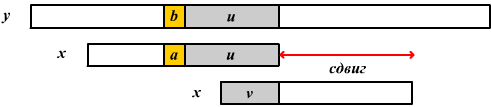
\includegraphics[width=0.7\linewidth]{img/10_1.png}
	\captionsetup{labelformat=empty}
	\caption{\textbf{Сдвиг хорошего суффикса}, вся подстрока u полностью встречается справа от символа c, отличного от символа a}
\end{figure}

\begin{figure}[h!]
	\centering
	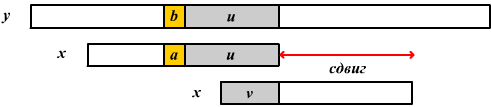
\includegraphics[width=0.7\linewidth]{img/10_1.png}
	\captionsetup{labelformat=empty}
	\caption{\textbf{Сдвиг хорошего суффикса}, только суффикс подстроки u повторно встречается в x.}
\end{figure}


\subsection{Эвристика стоп-символа}

На этапе инициализации составляется таблица плохих символов, в которой у каждого символа из алфавита отмечается последняя позиция его вхождения в шаблон.


\begin{figure}[h!]
	\centering
	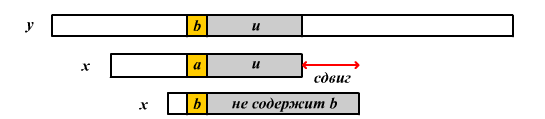
\includegraphics[width=0.7\linewidth]{img/10_3.png}
	\captionsetup{labelformat=empty}
	\caption{\textbf{Сдвиг плохого символа}, символ a входит в x.}
\end{figure}

\begin{figure}[h!]
	\centering
	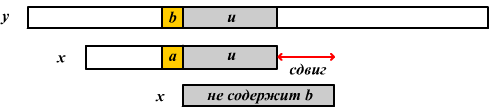
\includegraphics[width=0.7\linewidth]{img/10_4.png}
	\captionsetup{labelformat=empty}
	\caption{\textbf{Сдвиг плохого символа}, символ b не входит в x.}
\end{figure}


\textbf{Псевдокод алгоритма}

Константой $|\Sigma| = \sigma$  обозначим размер нашего алфавита.

\textbf{Функция для вычисления таблицы плохих символов}

%\begin{minted}{c}
%int[] preBmBc(char x[m]):
%	int table[S]
%	// Заполняем значением по умолчанию, равным длине шаблона
%	for i = 0...S- 1
%		table[i] = m
%	// Вычисление функции по определению
%	for i = 0 .. m - 2
%		table[x[i]] = m - 1 - i
%	return table
%\end{minted}
%
%\textbf{Функция, проверяющая, что подстрока $x[p..m-1]$является префиксом шаблона.} 
%Требуется $O(m - p)$ времени
%
%\begin{minted}{c}
%boolean isPrefix(char x[m], int p):
%	int j = 0
%	for i = p .. m - 1
%		if x[i] != x[j]
%			return False
%		j++
%	return True
%\end{minted}